\subsection{Cen�rio Edi��o \label{use_case_edicao}}

\begin{figure}[h|top]
 \centering
 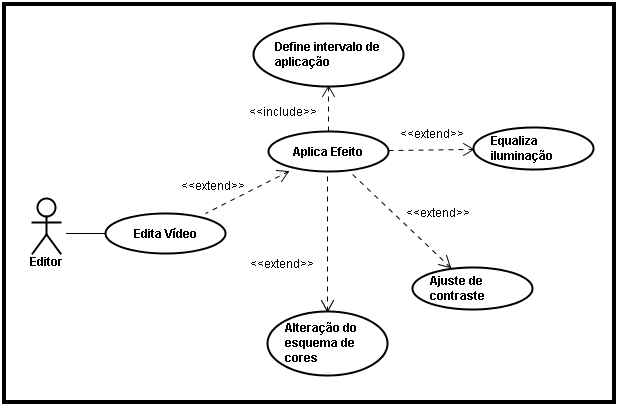
\includegraphics[width=1.0\linewidth]{imagens/use_case_edicao.png}
 \caption{Caso de Uso para cen�rio de edi��o de v�deo.}
 \label{img_use_case_edicao}
\end{figure}

\hspace*{0.65cm}A Figura \ref{img_use_case_edicao}

\subsubsection{Caso de uso: Aplica efeitos \label{use_case_aplica_efeito}}

\hspace*{1.25cm}\textbf{Cen�rio Principal:} O usu�rio aplica um ou
mais efeitos de edi��o no v�deo carregado.

\subsubsection{Caso de uso: Define intervalo de aplica��o \label{use_case_define_aplic}}

\hspace*{1.25cm}\textbf{Cen�rio Principal:} O usu�rio deve definir
qual ser� o trecho do v�deo em que dever� ser aplicado o efeito
selecionado. Por default, o sistema aplica o efeito na tomada que
estiver selecionada, ou no v�deo todo, caso n�o haja nenhuma tomada
selecionada.

\subsubsection{Caso de uso: Equaliza ilumina��o \label{use_case_iluminacao}}

\hspace*{1.25cm}\textbf{Cen�rio Principal:} O usu�rio poder�
realizar a equaliza��o da ilumina��o em uma tomada do v�deo. A qual
poder� ser autom�tica, ou frame a frame.

\subsubsection{Caso de uso: Ajuste de Contraste \label{use_case_contraste}}

\hspace*{1.25cm}\textbf{Cen�rio Principal:} O usu�rio poder�
realizar ajustes de contraste em uma tomada do v�deo.

\subsubsection{Caso de uso: Altera��o do Esquema de Cores \label{use_case_cores}}

\hspace*{1.25cm}\textbf{Cen�rio Principal:} O usu�rio aplica efeitos
para altera��o do esquema de cores do v�deo carregado ou de uma
tomada espec�fica do v�deo.
